\chapter{Router con QoS - WRR[1,1]}
\label{chap:conqoswrr11}

\tcolorbox[colback=yellow!20, colframe=yellow!50!black, title=Nota]
En este capítulo, como la proporción con WRR[1,1] es igual para ambas colas UDP, en muchos apartados
se da un único resultado para ambas colas, ya que el cálculo y resultado es el mismo para Afx1 que para 
Afx2. Cuando esto ocurre nos referimos a la cola genérica 'Afx'.
\endtcolorbox

\section{Longitud de cola del router}

\subsection{Calcula analíticamente cuántos paquetes habrá como máximo en la cola EF.}

\renewcommand{\theenumi}{\alph{enumi}}

La cola EF, que representa el flujo UDP, es manejada en este caso mediante \textit{Strict Priority Queueing},
por lo que podemos 'ignorar' las colas de paquetes UDP y simplemente calcular la tasa de salida con la
única restricción que supone limitar el tráfico EF a la tasa efectiva resultante de transmitir VoIP que, 
en este caso es de 76,8kbps, como se indica en el enunciado.


\[
R_{InVoIP} = \frac{1~\text{pkt}}{0,02~\text{s}} = 50 ~ \text{pkt/s}
\]

\[
R_{outVoIP} = \frac{76,8~\text{kb/s} \cdot 1000~\text{b/kb} \cdot \frac{1~\text{B}}{8~\text{b}}}{ 192~\text{B/pkt}} = 50~\text{pkt/s}
\]

\[
R_{InVoIP} = R_{outVoIP}
\]

Como la tasa de salida es igual a la de entrada, habrá como mucho un paquete VoIP en
cola en todo momento, ya que cada paquete se transmite al mismo tiempo que llega el siguiente.
Esto puede ratificarse al observar la línea verde, que representa la cola EF, en la figura \ref{fig:wrr11_tam}.

\begin{figure}[!ht]
    \centering
    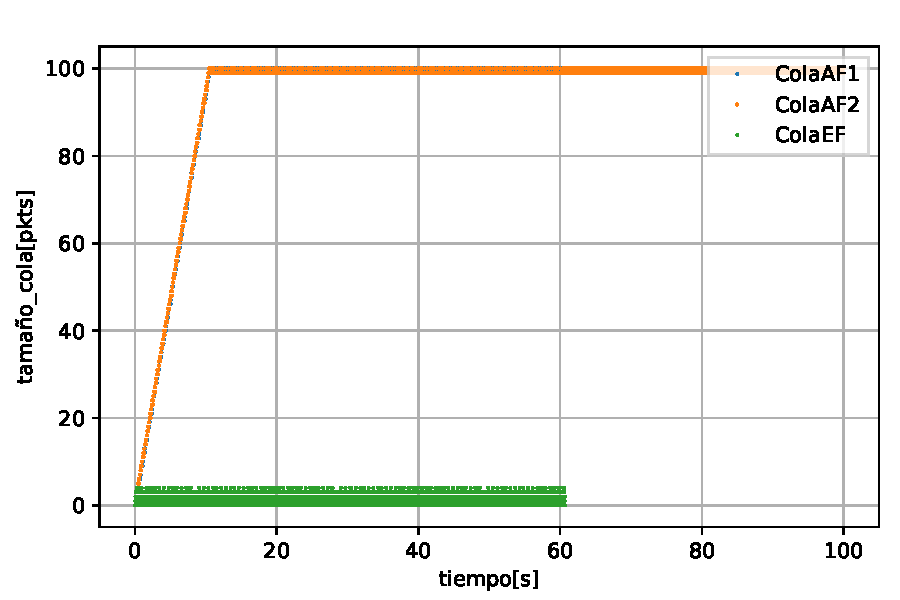
\includegraphics{graficas/DropTail/tamanho_cola_droptail.pdf}
    \caption{Longitud de la cola del router aplicando colas DropTail}
    \label{fig:wrr11_tam}
\end{figure}

\subsection{Mientras dura la transmisión del flujo VoIP:}
\begin{enumerate}
    \item Tasa de salida (en pkt/s y b/s) de cada cola AF1x y AF2x: \\
    \[
        \begin{aligned}
            R_{\text{OutUDP}}[b/s] &= R_{\text{Out}} - R_{\text{OutVoIP}} = 128~\text{kb/s} \cdot 1000~\text{b/kb} - 50~\text{pkt/s} \cdot 199~\text{B/pkt} \cdot 8~\text{b/B} \\
                              &= 48400~\text{b/s} \\
            R_{\text{OutUDP}}[pkt/s] &= 48400~\text{b/s} \cdot \frac{1~\text{B}}{8~\text{b}} \cdot \frac{1~\text{pkt}}{1000~\text{B}} = 6,05~\text{pkt/s} \\ \\
            R_{\text{OutAf1}}[b/s] &= p_{\text{Af1}} \cdot R_{\text{OutUDP}} = \frac{1}{2} \cdot 48400~\text{b/s} = 24200~\text{b/s} \\
            R_{\text{OutAf1}}[pkt/s] &= p_{\text{Af1}} \cdot R_{\text{OutUDP}} = \frac{1}{2} \cdot 6,05~\text{pkt/s} = 3,025~\text{pkt/s} \\ \\
        \end{aligned}
    \]
    \item Paquetes por segundo descartados a la entrada de cada cola:
    \[
        \label{eq:udp_paquetes_descartados_con_VoIP}
        \begin{aligned}
            R_{\text{InAfx}} &= \frac{1~\text{pkt}}{0,08~\text{s}} = 12,5~\text{pkt/s} \\ \\
            Pkt_{\text{DescAfx}} &= R_{\text{InAfx}} - R_{\text{OutAfx}} = 12,5~\text{pkt/s} - 3,025~\text{pkt/s} = 11,636~\text{pkt/s} \\
        \end{aligned}
    \]
    \item Tiempo de llenado de las colas AF1x y AF2x:
    \[
        \begin{aligned}
            t_{\text{FillAfx}} &= \frac{L}{R_{\text{InAfx}} - R_{\text{OutAfx}}} = \frac{100~\text{pkt}}{12,5~\text{pkt/s} - 3,025~\text{pkt/s}} = 9,475~\text{s} \\
        \end{aligned}
    \]
    El resultado de este apartado se puede que es correcto al contrastarlo con la figura \ref{fig:wrr11_tam}.

\end{enumerate}

\vspace{0,3cm}

\subsection{Para el caso en el que ya solo se están transmitiendo los dos flujos UDP, calcula la tasa de entrada [pkt/s] y
tasa de salida [pkt/s].}
La tasa de entrada no cambia. Como se indica en el enunciado, cada cola UDP recibe un paquete cada 80ms. \\
\[
    \begin{aligned}
        R_{\text{InAfx}} &= \frac{1~\text{pkt}}{0,08~\text{s}} = 12,5~\text{pkt/s} \\ \\
    \end{aligned}
\]
Por otra parte, ahora que no hay flujo VoIP (Y suponiendo cola EF vacía), las colas UDP pueden usar todo
el espacio del enlace router-servidor.
\[
    \begin{aligned}
        R_{\text{OutUDP}}[pkt/s] &= 128~\text{kb/s} \cdot 1000~\text{b/kb} \cdot \frac{1~\text{B}}{8~\text{b}} \cdot \frac{1~\text{pkt}}{1000~\text{B}} = 16~\text{pkt/s} \\
		R_{\text{OutAfx}}[pkt/s] &= p_{\text{Afx}} \cdot R_{\text{OutUDP}} = \frac{1}{2} \cdot 16~\text{b/s} = 8~\text{pkt/s} \\
    \end{aligned}
\]
Como se comprueba, el enlace sigue siendo insuficiente y las colas no se vaciarán mientras sigan llegando paquetes
ya que: \[R_{InAfx} > R_{outAfx}\].

\vspace{1cm}

\section{Tiempo en cola del router}

\subsection{Mientras dura la transmisión del flujo VoIP, calcula analíticamente el tiempo en cola de un paquete cuando
las colas AF1x y AF2x están llenas.}
\[
    \begin{aligned}
        t_{\text{qAfx}} &= \frac{L}{R_{\text{OutAfx}}} = \frac{100~\text{pkt}}{3,025~\text{pkt/s}}= 33,058~\text{s} \\
    \end{aligned}
\]

\vspace{0,3cm}

\subsection{Para el caso en el que ya solo se están transmitiendo los dos flujos UDP, calcula el tiempo medio en cola de
un paquete.}
\[
    \begin{aligned}
        t_{\text{qAfx}} &= \frac{L}{R_{\text{OutAfx}}} = \frac{100~\text{pkt}}{8~\text{pkt/s}}= 12,5~\text{s} \\
    \end{aligned}
\]

\vspace{1cm}

\section{Retardo extremo a extremo}

\subsection{¿Cambia algo la explicación con respecto al caso de Router sin QoS?}
La explicación es la misma que para el caso del router sin QoS aplicada. Las gráficas de \textit{end-to-end delay}
y tiempo de encolado son prácticamente idénticas debido a que, en el caso de esta práctica, el único segmento del 
sistema donde hay congestión y del que surjen todos los problemas es la conexión router-servidor. Además, el sistema
con el que se trabaja es bastante pequeño, haciendo que apenas se note el tiempo de viaje de los paquetes del origen 
a destino. Por tanto, es evidente ver que la práctica totalidad del retraso de los paquetes proeda del tiempo de 
espera en la cola con la que tratamos en estos ejercicios.

\vspace{1cm}

\section{Muestras VoIP perdidas y Paquetes VoIP perdidos}

\subsection{¿A qué se deben las muestras perdidas ahora? ¿Se pierde algún paquete VoIP?}

En este caso, las muestras perdidas son muy pocas gracias a aplicar técnicas de QoS. Las pocas muestras
que se pierden pueden ser debidas a ráfagas ocasionales de tráfico u otras situaciones inherentes a la naturaleza de la red.
De hecho, en este caso ya no se pierde ningún paquete en la transmisión.

\begin{figure}[!ht]
    \centering
    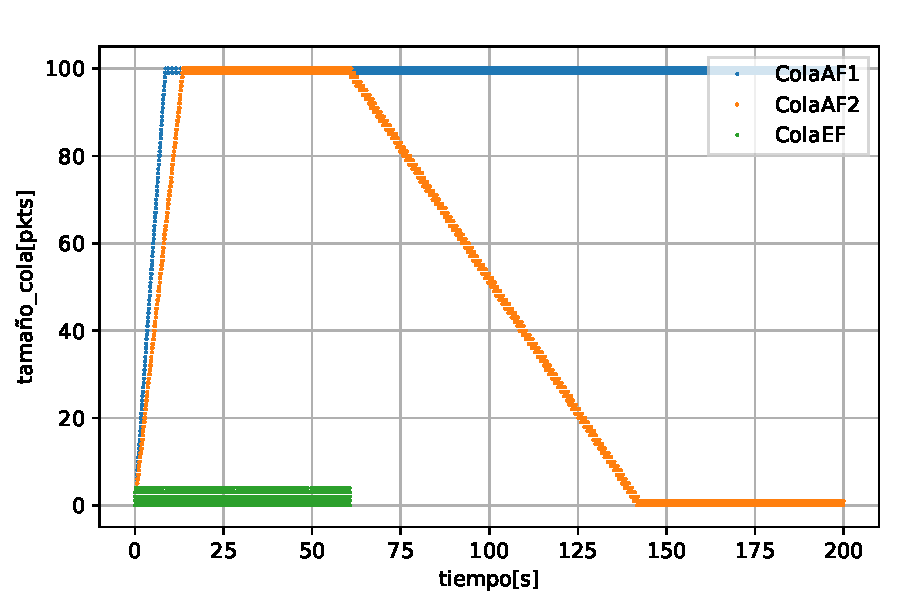
\includegraphics{graficas/WRR/tamao_cola_wrr.pdf}
    \caption{Muestras perdidas en router con WRR[1,1]}
    \label{fig:wrr16_lostsamples}
\end{figure}